\documentclass{article}
\usepackage{hyperref,amsmath,amsthm,xcolor,graphicx}




\def\imp{\Rightarrow}
\newcommand{\rstar}[1]{#1^*}
\newcommand{\rplus}[1]{#1^+}
\newcommand{\reqv}[1]{#1^\sim}
\newcommand{\toplus}{\rplus\to}
\newcommand{\tostar}{\rstar\to}
\newcommand{\tobeta}{\to_\beta}
\newcommand{\tobetaplus}{\to^+_\beta}
\newcommand{\tobetastar}{\to^*_\beta}
\newcommand{\tobetap}{\to_{p}}
\newcommand{\tobetapplus}{\to^+_{p}}
\newcommand{\tobetapstar}{\to^*_{p}}
\newcommand{\betaeqv}{\sim_\beta}
\newcommand{\toeqv}{\reqv\to}
\newcommand{\neglow}{\neg\,}

\newcommand{\indrule}[2]{\begin{array}{l} #1 \\ \hline #2\end{array}}
\newcommand{\ruleh}[2]{\begin{array}{c} #1 \\ \hline #2\end{array}}
\newcommand{\rulev}[2]{\begin{array}{l} #1 \\ \hline #2\end{array}}



\title{Lambda Calculus - Step by Step}
\author{Helmut Brandl}
\date{}



\begin{document}
\maketitle

\tableofcontents

\theoremstyle{definition} \newtheorem{definition}{Definition}[section]
\theoremstyle{definition} \newtheorem{theorem}{Theorem}[section]
\theoremstyle{definition} \newtheorem{lemma}{Lemma}[section]

\section{Motivation}

This is a picture of David
Hilbert: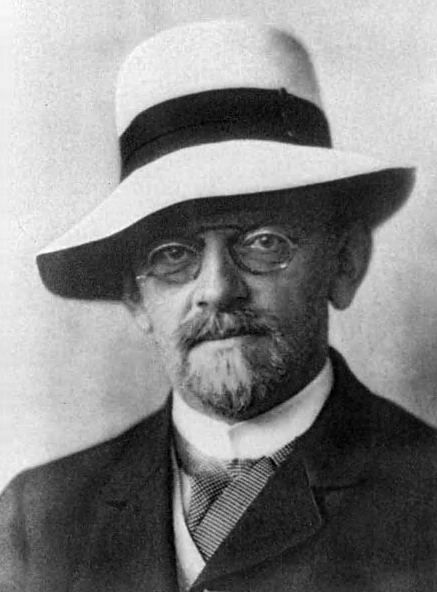
\includegraphics[scale=0.2,angle=90]{../img/hilbert.jpg} This is the text
which follows.


\section{Inductive Sets and Relations}


\begin{definition} The \emph{transitive closure} $\rplus{r}$ of a relation $r$ is
  defined by the rules
1.~$\rulev{r(a,b)}{\rplus{r}(a,b)}$,
2.~$\rulev{\rplus{r}(a,b) \\ r(b,c)}{\rplus{r}(a,c)}$
\end{definition}

\begin{definition} The \emph{reflexive transitive closure} $\rstar{r}$ of a relation $r$ is
  defined by the rules
1.~$\rulev{}{\rstar{r}(a,a)}$,
2.~$\rulev{\rstar{r}(a,b) \\ r(b,c)}{\rstar{r}(a,c)}$
\end{definition}

\begin{definition} The \emph{equivalence closure} $\reqv{r}$ of a relation $r$ is
  defined by the rules
  1.~$\rulev{}{\reqv{r}(a,a)}$,
  2.~$\rulev{\reqv{r}(a,b)
    \\ r(b,c)} {\reqv{r}(a,c)}$,
  3.~$\rulev{\reqv{r}(a,b) \\ r(c,b)} {\reqv{r}(a,c)}$
\end{definition}

\begin{theorem}
  All closures are increasing $r \subseteq r^c$, monotonic
  $r \subseteq s \imp r^c \subseteq s^c$ and idempotent $r^{cc} = r$. Proof
  e.g. for the reflexive transitive closure. TBD.
\end{theorem}

\begin{theorem}
A relation $s$ which satisfies $r \subseteq s \subseteq r^c$ has the same closure
as $r$ i.e. $r^c = s^c$. Proof:
  \begin{itemize}
  \item $r^c \subseteq s^c$ by monotonicity.
  \item $s^c \subseteq r^c$: $s^c \subseteq r^{cc}$ by
    monotonicity and then use idempotence to conclude $s^c \subseteq r^c$.
  \end{itemize}
\end{theorem}



Theorems: $\rplus{r}$ is transitive, $\rstar{r}$ is transitive, $\reqv{r}$ is
symmetric, $\rplus{r}\subseteq\rstar{r}$, $r$ reflexive $\imp \rplus{r} =
\rstar{r}$.


\begin{definition}
  $a$ is a \emph{terminal element} of the relation $\to$ if it has no
  successor i.e. $\forall b: \neglow a \to b$.
\end{definition}

\begin{definition}
  $a$ is a \emph{terminating element} of the relation $\to$ if there is a path
  to a terminal element $b$ i.e. $a \tostar b$.
\end{definition}

\begin{definition}
A relation $\to$ is a \emph{diamond} if for all $a$, $b$ and $c$ there exists a $d$
such that
$
  \begin{matrix}
    a & \to & b \\
    \downarrow & & \downarrow \\
    c & \to & \exists d
  \end{matrix}
$
\end{definition}


\begin{definition}
  A relation $r$ is \emph{confluent} if $\rstar{r}$ is a diamond.
\end{definition}

\begin{theorem} In a confluent relation $r$ all two $r$-equivalent elements
  meet at some common element
  $
  \begin{matrix}
    a & \reqv\to & b \\
    & \rstar\searrow & \downarrow_*\\
    & & \exists c
  \end{matrix}
  $.
  Proof by induction on $a\reqv\to b$.
  \begin{enumerate}

  \item $a = b$. Trivial. Take $c = a$.

  \item
    $\begin{matrix}
      a & \reqv\to & b & \to & c\\
      & \rstar\searrow & \downarrow_*  & & \downarrow_*\\
      & & d? & \rstar\to & e?
    \end{matrix}$.
    $d$ exists by induction hypothesis, $e$ exists by confluence.

  \item
    $
    \begin{matrix}
      a & \reqv\to & b & \gets & c\\
      & \rstar\searrow & \downarrow_*  & & \downarrow_*\\
      & & d? & \rstar\to & e?
    \end{matrix}
    $.
    $d$ exists by induction hypothesis, $e$ exists by confluence.
  \end{enumerate}
\end{theorem}

Definition: $a$ is a terminal element of $r$ if $\neg r(a,b)$ for all $b$.

Definition: Set $\overline T$ of terminating elements of a relation $r$:
$\rulev{a\in T}{a\in \overline T}$, $\rulev{r(a,b) \\ b\in\overline T}{a\in
  \overline T}$ where $T$ is the set of terminal elements. By definition: For
all terminating elements $a$ there is a terminal element $b$ with $\rstar
r(a,b)$.

Theorem: In a confluent relation all terminating elements have a unique
terminal element. Proof: Suppose there are two terminal elements $b$ and $c$
for the terminating element $a$. By definition there must be a $d$ such that
$\begin{matrix} a & \tostar & b \\
  \downarrow_* & & \downarrow_* \\
  c & \tostar & d
\end{matrix}$
which contradicts the assumption that $b$ and $c$ are terminal.


Theorem: In a confluent relation $r$ two $r$-equivalent terminating elements have the same
terminal element.
Proof: Assume $a \reqv\to b$ and $a \to_* c$ and $b \to_* d$
where $c$ and $d$ are different terminal elements. Prove by induction on $a
\reqv\to b$. Case (a): $a=b$. By the previous theorem the terminal element
must be unique. Contradiction. Case (b): $a \reqv\to b$ and $b \to c$. By
induction hypothesis $a$ and $b$ must have the same terminal element.

Theorem: The reflexive transitive closure of a diamond is a diamond (stripe
lemma).
Proof:
\begin{itemize}
\item Lemma: Let $\to$ be a diamond. Then
$\begin{matrix}
a & \to_* & b \\
\downarrow & & \downarrow \\
c & \to_* & \exists d
  \end{matrix}$.
Proof by induction on $a \to_* b$.
\begin{itemize}
\item Case (a): $a = b$. Trivial, take $d=c$.
\item Case (b):
$\begin{matrix}
a & \to_* & b & \to & c\\
\downarrow & & \downarrow & & \downarrow\\
d & \to_* & e? & \to & f?
\end{matrix}$. $e$ exists by the induction hypothesis, $f$ exists because
$\to$ is a diamond.
\end{itemize}

\item Theorem:  Let $\to$ be a diamond. Then
$\begin{matrix}
a & \to_* & b \\
\downarrow_* & & \downarrow_* \\
c & \to_* & \exists d
  \end{matrix}$. Proof by induction on $a \to_* c$.
\begin{itemize}
\item Case (a): $a = b$. Trivial, take $d=c$.
\item Case (b):
$\begin{matrix}
a & \to_* & b\\
\downarrow_* & & \downarrow_* \\
c & \to_* & e?  \\
\downarrow & & \downarrow \\
d & \to_* & f?
\end{matrix}$. $e$ exists by induction hypothesis, $f$ exists by the previous lemma.
\end{itemize}
\end{itemize}



\section{Lambda Terms}

\begin{definition}
  Let $x$ range over a countably infinite set of variable names then the set
  of lambda terms is defined by the grammar $$t ::= x \mid t t \mid \lambda x. t$$.
\end{definition}

A lambda term is either a variable $x$, an application $a b$ (the term $a$
applied to the term $b$) or an abstraction $\lambda x.a$.

We use the convention that application is left associative i.e. $a b c$ is
parsed as $(a b) c$.

Nested lambda abstractions $\lambda x. \lambda y. \ldots . t$ are abbreviated
as $\lambda x y \ldots . t$

\begin{definition}
  The set of free variables $FV(t)$ of a lambda term $t$ is defined by
  $$FV(t) :=
  \begin{cases} FV(x) &= \{x\} \\
     FV(a b) &= FV(a) \cup FV(b) \\
     FV(\lambda x. t) &= FV(t) - \{x\}
   \end{cases}
   $$
\end{definition}

The variable $x$ in the term $t$ of the abstraction $\lambda x.t$ is a bound
variable. Bound variables can be renamed arbitrarily. We consider terms equal
which have just different namings of bound variables. E.g. the term $\lambda
x.x$ and $\lambda y.y$ are equal.

\begin{definition}
  The variable substitution $a[x:=t]$ is defined by
  $$a[x:=t]~:=
  \begin{cases} x[x:=t]  &:= t \\
    y[x:=t] &:= y \quad \text{for}\quad x \ne y \\
    (a b)[x:=t] &:= a[x:=t] \, b[x:=t] \\
    (\lambda y.a)[x:=t]  &:= \lambda y. a[x:=t] \quad\text{for}\quad x \ne y
    \land y \notin FV(t)
   \end{cases}
   $$
\end{definition}

\begin{definition} \emph{Beta reduction} $\tobeta$ is a relation defined over lambda
  terms by the rules
  \begin{enumerate}
  \item $(\lambda x.a) b \tobeta a[x := b]$
  \item $\rulev{a\tobeta b}{a c \tobeta b c}$
  \item $\rulev{b\tobeta c}{a b \tobeta a c}$
  \item $\rulev{a \tobeta b}{\lambda x.a \tobeta \lambda x.b}$
  \end{enumerate}
\end{definition}

\section{Church Rosser - Confluence}

\begin{definition} \emph{Parallel beta reduction} $\tobetap$ is a relation
  defined over lambda terms by the rules
  \begin{enumerate}
  \item $a \tobetap a$
  \item $\rulev{a \tobetap b} {\lambda x.a \tobetap \lambda x.b}$
  \item $\rulev{a\tobetap c \\ b \tobetap d}{a b \tobeta c d}$
  \item $\rulev{a\tobetap c \\ b \tobetap d}{(\lambda x.a) b \tobetap c[x := d]}$
  \end{enumerate}
\end{definition}

In order to prove that $\tobetap$ is a diamond we need some lemmas.

\begin{lemma}
  Parallel beta reduction preserves abstractions i.e.
  $\lambda x.a \tobetap c \imp \exists b : a \tobetap b \land c = \lambda
  x.b$. Proof by induction on $\tobetap$.
  \begin{enumerate}
  \item $c = \lambda x.a$. Trivial. Take $b = a$.
  \item $\lambda x.a \tobetap \lambda x.b$ with $a \tobetap b$. Trivial. Take $b$.
  \item The case $\lambda x.a = t u$ is syntactically impossible. Abstraction
    and application are different.
  \item The case $\lambda x.a = (\lambda x.u) v$ is syntactically
    impossible. Abstraction and application are different.
  \end{enumerate}
\end{lemma}


\begin{lemma}
  $t \tobetap u \imp a[x := t] \tobetap a[x := u]$. Proof TBD.
\end{lemma}

\begin{lemma}
  $a \tobetap c \land b \tobetap d  \imp a[x := b] \tobetap c[x := d]$. Proof TBD.
\end{lemma}


\section{Reduction Strategies}

\section{Computations}

\section{Undecidability}


\begin{thebibliography}{99}

\bibitem{church1936} Church, A. (1936). An unsolvable problem of elementary number theory, American
Journal of Mathematics 58, pp. 354–363.

\bibitem{chuchrosser1936} Church, A., Rosser, J. B.: Some Properties of Conversion, Trans. Amer. Math. Soc., 39, 1936, 472–482.


\bibitem{goedel1931} Kurt Gödel (1931). Über formal unentscheidbare Sätze der
  Principia Mathematica und verwandter Systeme I, Monatshefte für Mathematik
  und Physik, vol. 38 (1931), pp. 173-198.

\bibitem{schoenfinkel1924} Schönfinkel, M. (1924). Über die Bausteine der mathematische Logik, Mathematische
Annalen 92, pp. 305–316.

\bibitem{turing1936} Turing, A.M. (1936/7). On computable numbers, with an application to the
Entscheidungsproblem, Proceedings of the London Mathematical Society
42, pp. 230–265.

\end{thebibliography}


\end{document}
